\section{Marco Teórico}

\subsection{Sistemas de referencia}

Para describir la dinámica orbital, de actitud y el diseño del ADCS, es necesario la definición de los marcos de referencia a utilizar. Su selección obedece a criterios descritos a continuación.

\begin{itemize}
	\item \textbf{Sistema de referencia body o del cuerpo \cite{ref21}}: La dinámica relativa de actitud se describe con respecto al marco de referencia del cuerpo en el CubeSat, desde la cual se realizan las mediciones, debido a que los sensores de actitud están fijados a su cuerpo. Para los marcos de referencia del cuerpo, el eje z apunta en la dirección del momento de inercia más alto, y los ejes x e y son paralelos a los vectores de área de las caras de la nave espacial, apuntando todos en las direcciones principales del satélite, como se observa gráficamente en la Figura~\ref{fig:body}.
	
	\begin{figure}[h]
		\centering    
		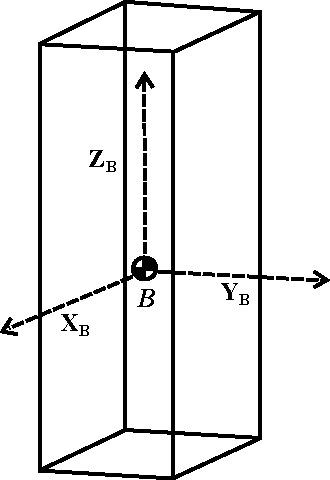
\includegraphics[width=0.28\textwidth]{body.pdf}
		\caption{Marco de referencia del cuerpo (Elaboración propia).}
		\label{fig:body}
	\end{figure}
	
	\item \textbf{Sistema de referencia inercial \cite{ref21,ref22}}: El Sistema de referencia inercial utilizado es el Earth Centered Inertial (ECI) debido a la necesidad de obtener vectores respecto a un marco de referencia no rotativo (asumiendo problema de dos cuerpos entre la Tierra y el satélite). El eje X apunta en la dirección del equinoccio de primavera. El plano XY es el plano ecuatorial de la Tierra, y el eje Z coincide con el eje de rotación de la Tierra y apunta hacia el norte. Este sistema de referencia se puede apreciar en la Figura~\ref{fig:ECI}.
	
	\begin{figure}[H]
		\centering    
		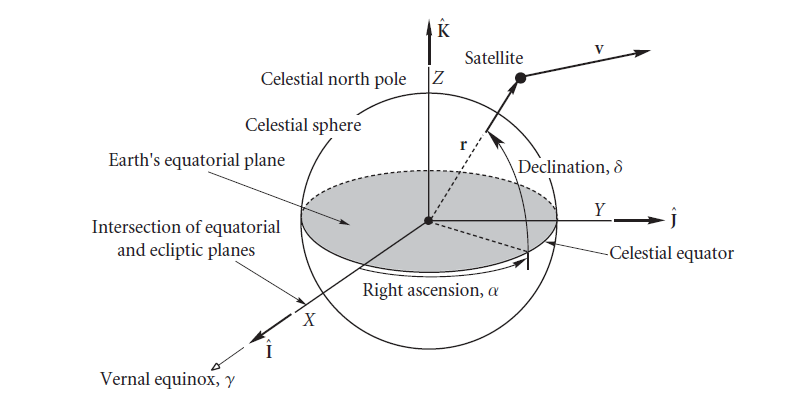
\includegraphics[width=0.8\textwidth]{ECI.png}
		\caption{Marco de referencia inercial ECI \cite{ref22}.}
		\label{fig:ECI}
	\end{figure}
	
	\item \textbf{Sistema de referencia LVLH o Roll-Pitch-Yaw  \cite{ref23}}: Se define un sistema coordenado que mantiene su orientación relativa a la Tierra a medida que la nave espacial se mueve en su órbita. Estas coordenadas son conocidas como roll, pitch y yaw (RPY), \textit{Local Vertical Local Horizontal} (LVLH) u orbital como también será llamada en este trabajo y se ilustra en la Figura~\ref{fig:RPY}. En este sistema, el eje yaw se dirige hacia el nadir (es decir, hacia el centro de la Tierra), el eje pitch se dirige hacia la normal negativa de la órbita, y el eje roll es perpendicular a los otros dos, tal y como se muestra en la Ecuación~\ref{eq:RPY}. Se utilizará este Sistema de referencia para notar la posición ideal de la carga útil.
	 \begin{equation}
		\hat{R} = \hat{P} \times \hat{Y}
		\label{eq:RPY}
	\end{equation} 


	\begin{figure}[H]
		\centering    
		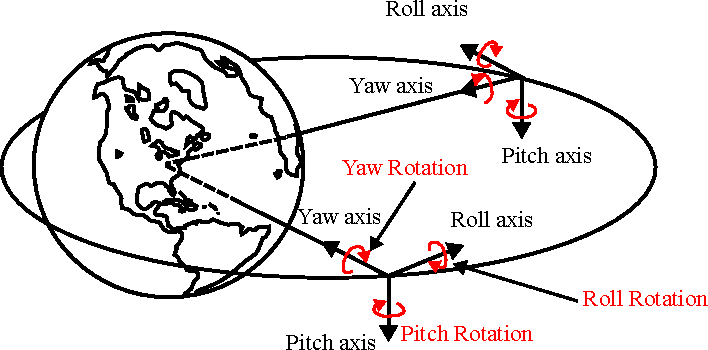
\includegraphics[width=0.6\textwidth]{RPY.pdf}
		\caption{Marco de referencia inercial RPY \cite{ref23}.}
		\label{fig:RPY}
	\end{figure}	
	
\end{itemize}


\subsection{Dinámica orbital}

Para el modelamiento de la suite de simulación se debe conocer el significado de los parámetros orbitales que se entregara como entrada, así como las ecuaciones que gobiernan el movimiento del satélite a través de la Tierra y las perturbaciones presentes a baja altura.

\subsubsection{Parámetros orbitales}

Si la masa de un satélite se considera insignificante en comparación con la masa de la Tierra, y bajo el supuesto de que la Tierra es esféricamente simétrica, la aceleración \( \ddot{\mathbf{r}} \) de un satélite está dado por la ley de gravedad de Newton descrita a continuación:

\begin{equation}
	\ddot{\mathbf{r}} = -\frac{GM_E}{r^3} \mathbf{r}
	\label{eq:Newton}
\end{equation}

Donde $\mathbf{r}$ es el vector posición entre el satélite y la Tierra y $GM_E$ es conocida como la constante de gravitacional de la Tierra y está dada por:

\begin{equation}
	\mu = {GM_E} = 398600,4418  [\frac{{km}^3}{{s}^2}]
	\label{eq:cteGrav}
\end{equation}

Al resolver la Ecuación~\ref{eq:Newton}, se obtiene la posición y la velocidad del del satélite respecto a la Tierra en cualquier instante de tiempo dependiendo del sistema de referencia a utilizar. Si bien se tiene una cuantificación del posicionamiento y el movimiento del satélite, generalmente se utiliza otra caracterización para definir la órbita, utilizando los elementos keplerianos, los cuales se presentan en la Figura~\ref{fig:kepler}.

\begin{figure}[H]
	\centering    
	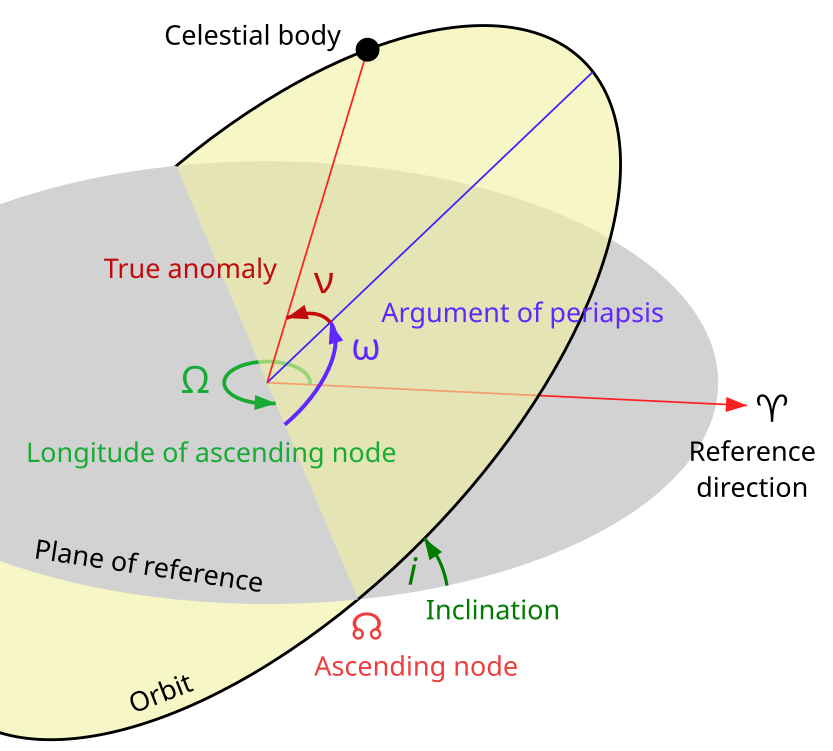
\includegraphics[width=0.45\textwidth]{keplerianos.png}
	\caption{Elementos keplerianos \cite{ref24}.}
	\label{fig:kepler}
\end{figure}

Dichos elementos se definen brevemente a continuación, los que se pueden determinar desde la posición y la velocidad del satélite respecto a la Tierra mediante relaciones matemáticas obtenidas en \cite{ref22}.


\begin{itemize}
	\item \textbf{Excentricidad (e)}: Describe el alargamiento de la órbita. Si presenta valores entre 0 y 1 tendrá forma de elipse. Si es igual a 0 representa una órbita circular, mientras que si es igual a 1 tiene forma de parábola. Para casos mayores a 1 se presentan orbitas de trayectoria hiperbólica.
	
	\item \textbf{Semieje mayor (a)}: Es la distancia entre el periapsis (distancia más cercana entre el satélite y la Tierra) y el apoapsis (distancia más lejana entre el satélite y la Tierra) dividido por 2. Representa el radio para orbitas circulares.
	
	\item \textbf{Inclinación (i)}: Inclinación vertical de la elipse con respecto al plano de referencia (plano ecuatorial).
	
	\item \textbf{Right Ascension of the Ascending Node (RAAN $\Omega$)}: Inclinación vertical de la elipse con respecto al plano de referencia (plano ecuatorial).	
	
	\item \textbf{Argumento del periapsis ($\omega$)}: Se define la orientación de la elipse en el plano orbital, como un ángulo medido desde el nodo ascendente a la periapsis.
	
	\item \textbf{Anomalía verdadera  ($\nu$)}: Define la posición del cuerpo orbitante a lo largo de la elipse en un tiempo específico.
\end{itemize}

\subsubsection{Perturbaciones presentes en LEO}

Existen perturbaciones en el espacio que afectan a los satélites en órbita, de las cuales algunas tienen más relevancia a bajas altura respecto de la Tierra. Estas se muestran a continuación:

\textbf{Gravedad no esférica \cite{ref25}}: La Tierra no es una esfera perfecta y la masa se distribuye de manera no uniforme. A diferencia de las simplificaciones que se aplican a menudo en órbitas altas, donde la influencia de la Tierra se aproxima a una esfera, en LEO la distribución irregular de la masa terrestre y las variaciones en la altitud pueden generar perturbaciones significativas en las trayectorias de los satélites. Por lo tanto, como la fuerza de gravedad depende directamente de la masa, el campo gravitatorio reflejará esta falta de uniformidad.

Para lograr modelar la gravedad no esférica se utiliza una expansión armónica esférica, con modelos como el geopotencial que descompone el campo gravitatorio terrestre en una serie de términos, cada uno correspondiente a una armonía esférica y su respectiva magnitud. Dentro de los coeficientes utilizados dentro del modelo recién mencionado están los “J”, siendo el J2 el principal para modelar el achatamiento de la Tierra. Otros J como el J3, J4, etc., modelan a mayor detalle la distribución másica de la Tierra.

\textbf{Efectos atmosféricos \cite{ref26}}: Los efectos del arrastre y el oxígeno atómico (O) tienen implicancias para los satélites de baja altura (menor a 600 km). El arrastre se define como una fuerza resistiva que actúa sobre un objeto en movimiento a través de un fluido y tiende a disminuir su velocidad, cuyas implicancias son que acorta la vida útil del satélite. El arrastre depende de la densidad, la velocidad y también variará según cómo cambie la atmósfera (se expanda o se contraiga) debido a la variación en la actividad sola. 

Por otro lado, debido a que en la atmosfera superior existe una mayor radiación, esto hace que se disocien los átomos de $O_{2}$ a O, los cuales son muy reactivos y potencialmente dañinos, degradando las superficies del CubeSat e interfiriendo con los sensores para la determinación de actitud.

\subsection{Cinemática y dinámica de actitud}

Para la cinemática y dinámica de actitud, el satélite ya no se asume como una partícula perturbada (como en el caso de la dinámica orbital), sino como un cuerpo rígido con masa. Con esto aparecen conceptos que serán definidos en esta sección.

\subsubsection{Actitud de un satélite y sus representaciones}

La actitud de un satélite se refiere a la orientación o posición que mantiene en el espacio mientras órbita alrededor de la Tierra u otro cuerpo celeste. Para describir esta actitud, se utilizan diversas representaciones matemáticas que permiten definir de manera precisa su orientación en el marco de referencia del cuerpo respecto al inercial, las cuales se presentan a continuación \cite{ref23}:


\begin{itemize}
	\item \textbf{Direction Cosine Matrix (DCM)}: Esta parametrización utiliza una matriz 3x3 para representar la orientación del satélite en relación con un sistema de referencia fijo. La matriz contiene nueve elementos que son los cosenos directores de los ejes del satélite en relación con los ejes de referencia. Es una representación matemáticamente precisa pero no es tan intuitiva como otras. Dicha representación se visualiza en la Figura~\ref{fig:DCM}.
	
	\begin{figure}[H]
		\centering    
		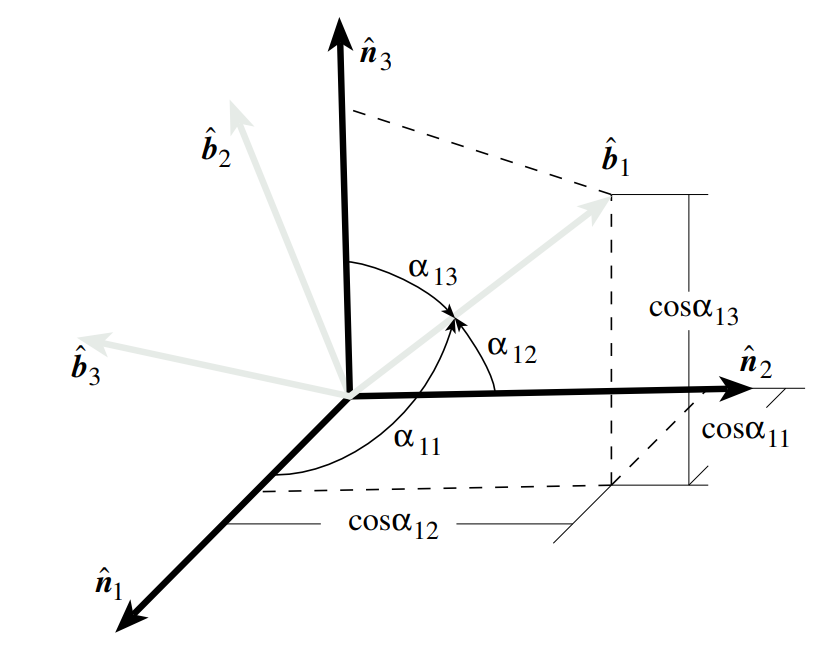
\includegraphics[width=0.45\textwidth]{DCM.png}
		\caption{Representación gráfica de la primera fila de la matriz de cosenos directores \cite{ref27}.}
		\label{fig:DCM}
	\end{figure}
	
	\item \textbf{Euler axis/angle}: En esta parametrización, se utiliza un vector tridimensional (el eje de Euler) junto con un ángulo para describir la orientación. El vector de Euler define el eje de rotación, mientras que el ángulo especifica la magnitud de la rotación alrededor de ese eje, como se muestra en la Figura~\ref{fig:axis_angle}. Es útil para representar giros simples y es intuitiva. 
	
	\begin{figure}[H]
		\centering    
		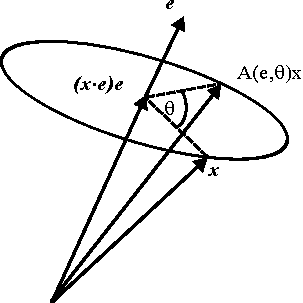
\includegraphics[width=0.3\textwidth]{axis_angle.pdf}
		\caption{Representación de un cambio de orientación en Euler axis/angle de x \cite{ref25}.}
		\label{fig:axis_angle}
	\end{figure}	
	
	\item \textbf{Euler angles}: Esta parametrización describe la orientación mediante tres ángulos, generalmente llamados phi ($\phi$), theta ($\theta$) y psi ($\psi$), que representan las rotaciones en torno a los ejes específicos (por ejemplo, X, Y y Z). Se presenta en la Figura~\ref{fig:euler_angles} las rotaciones realizadas por esta parametrización. 
	
	\begin{figure}[H]
		\centering    
		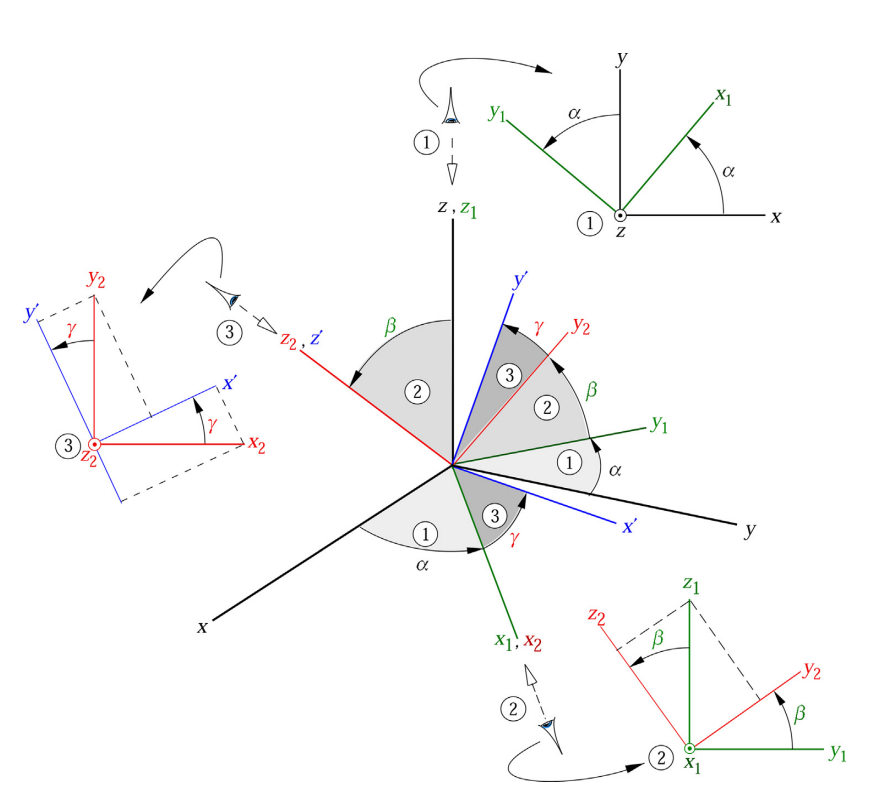
\includegraphics[width=0.6\textwidth]{euler_angles.png}
		\caption{Secuencia clásica de Euler de tres rotaciones que transforman xyz en x’y’z’ \cite{ref22}.}
		\label{fig:euler_angles}
	\end{figure}
	
	\item \textbf{Cuaternión}: Esta parametrización utiliza cuatro parámetros para representar la orientación, siendo tres de estas vectoriales y una escalar. Se discutirá más a fondo en la siguiente sección. 			
\end{itemize}

\subsubsection{Cuaterniones y cinemática de cuaterniones}

En este trabajo, la parametrización seleccionada para la descripción de la actitud es el cuaternión. Los cuaterniones tienen múltiples ventajas en comparación con otras parametrizaciones de actitud. Por ejemplo, en la parametrización de ángulos de Euler, la propagación de la actitud no es suave. Sin embargo, esta suavidad es fundamental para el correcto funcionamiento de métodos de estimación como el Filtro de Kalman \cite{ref23}.

Por otro lado, la desventaja de la parametrización de la matriz de cosenos directores es que conduce a una descripción de la actitud utilizando nueve elementos no independientes, y cumple con seis restricciones impuestas por la ortogonalidad de la matriz de actitud que son redundantes.
La cantidad mínima de elementos que se pueden utilizar para describir la actitud sin singularidades son cuatro. A partir del hecho de que cualquier rotación puede describirse utilizando un solo eje de rotación y un ángulo que describe la rotación alrededor de este eje, el cuaternión se define mediante 4 elementos, con una parte vectorial y una parte escalar como se muestra a continuación \cite{ref22}:

\begin{equation}
	\hat{q} = \begin{bmatrix}
		q_0 \\
		q_1 \\
		q_2 \\
		q_3
	\end{bmatrix}
	= \begin{bmatrix}
		\mathbf{q} \\
		q_3
	\end{bmatrix}
	= \begin{bmatrix}
		\sin\left(\frac{\theta}{2}\right) \hat{u} \\
		\cos\left(\frac{\theta}{2}\right)
	\end{bmatrix}
	\label{eq:cin_quat}
\end{equation}

La expresión \( \mathbf{q} \) es la parte vectorial \( \mathbf{q} = q_0 \hat{i} + q_1 \hat{j} + q_2 \hat{k} \), y \( q_3 \) es la parte escalar. La representación mostrada corresponde a un cuaternión pasivo, el cual se utiliza para rotar el sistema de coordenadas en sí (sin rotar el vector). Si se desea rotar el vector sin rotar el sistema de coordenadas, se utiliza un cuaternión activo, y se obtiene cambiando la componente escalar al inicio, tal y como se muestra en la siguiente expresión:

\[
\hat{q} = \begin{bmatrix}
	q_3 \\
	q_0 \\
	q_1 \\
	q_2
\end{bmatrix}
= \begin{bmatrix}
	q_3 \\
	\mathbf{q}
\end{bmatrix}
\]

Sabiendo esto, se puede definir la cinemática de la actitud del satélite utilizando cuaterniones mediante la Ecuación ~\ref{eq:cin_omega}, sabiendo que \( \omega_0 \), \( \omega_1 \) y \( \omega_2 \) son las velocidades angulares en el marco de referencia cuerpo del satélite:

\begin{equation}
	\frac{d\hat{q}}{dt} = \frac{1}{2}
	\begin{bmatrix}
		0 & -\omega_2 & \omega_1 & -\omega_0 \\
		\omega_2 & 0 & -\omega_0 & -\omega_1 \\
		-\omega_1 & \omega_0 & 0 & -\omega_2 \\
		\omega_0 & \omega_1 & \omega_2 & 0
	\end{bmatrix}
	\hat{q}
	\label{eq:cin_omega}
\end{equation}

Además, se tiene la multiplicación de cuaterniones, la cual será útil para representar las rotaciones entre los sistemas de referencia y aproximaciones discretas que utilizan esta operación, la cual se representa en la Ecuación~\ref{eq:quat_mult}:

\begin{equation}
	\hat{q} \cdot \hat{r} =
	\begin{bmatrix}
		q_3 r_0 + q_0 r_3 + q_1 r_2 - q_2 r_1 \\
		q_3 r_1 + q_1 r_3 + q_2 r_0 - q_0 r_2 \\
		q_3 r_2 + q_2 r_3 + q_0 r_1 - q_1 r_0 \\
		q_3 r_3 - q_0 r_0 - q_1 r_1 - q_2 r_2
	\end{bmatrix}
	\label{eq:quat_mult}
\end{equation}

Si bien esta parametrización no tiene una representación física obvia, se puede describir la rotación del satélite a través del tiempo mediante un integrador numérico, sabiendo la condición inicial tanto del cuaternión como de la velocidad angular.

\subsubsection{Dinámica de actitud}

La ecuación que describe la variación del vector momento angular a través del tiempo para un torque aplicado en un marco de referencia del cuerpo representa la dinámica de actitud y se muestra en la Ecuación~\ref{eq:vect_dot} \cite{ref22}:

\begin{equation}
	I \frac{d\boldsymbol{\omega}}{dt} = - \boldsymbol{\omega} \times I \boldsymbol{\omega} + \boldsymbol{\tau}
	\label{eq:vect_dot}
\end{equation}

Sabiendo que \( \boldsymbol{\omega} \) es el vector de velocidad angular instantánea en el cuerpo, \( I \) son los momentos principales de inercia y \( \boldsymbol{\tau} \) son los torques aplicados, esta ecuación se puede representar también según sus componentes en \( i \), \( j \) y \( k \):

\[
\dot{\omega}_0 = \frac{\omega_1 \omega_2 (I_y - I_z)}{I_x} + \frac{\tau_x}{I_x}
\]
\[
\dot{\omega}_1 = \frac{\omega_0 \omega_2 (I_x - I_z)}{I_y} + \frac{\tau_y}{I_y}
\]
\[
\dot{\omega}_2 = \frac{\omega_0 \omega_1 (I_x - I_y)}{I_z} + \frac{\tau_z}{I_z}
\]

Los torques externos son los provocados por los actuadores y por perturbaciones externas en orbitas de baja altura. Las ultimas mencionadas generalmente se simplifican a relaciones para el peor de los casos analizados. Estas perturbaciones que afectan a la dinámica rotacional del satélite son cuatro y se discuten a fondo en el Anexo \ref{ap:Z2}.

\subsection{Subsistema de determinación y control de actitud}

El subsistema de determinación y control de actitud de un CubeSat es el responsable de determinar su orientación en el espacio y controlarla respecto a un objetivo durante un periodo específico. También se requiere para sobrevivir en el entorno espacial, controlando el satélite en orientaciones tales que se genere energía apuntando las celdas fotovoltaicas hacia el sol.

El proceso para poder describir el movimiento del satélite se describe en tres pasos o procesos los cuales son llamados Guidance, Navigation and Control (GNC). Cada uno se describe según los componentes del ADCS, como se muestra a continuación \cite{ref28}:

\begin{itemize}
	\item Navigation: Es el primer paso por seguir, y determina la actitud del satélite y la tasa de rotación mediante los sensores tanto inerciales como de medición externa. Responde a la pregunta: ¿Dónde está el satélite?
	\item Guidance: Al determinar la actitud con los sensores, se utilizan algoritmos de determinación de actitud para estimar la orientación tanto inicial como a través del tiempo, para posteriormente utilizar algoritmos de determinación de actitud para estimar la orientación del satélite. Responde a la pregunta: ¿Hacia dónde quiere ir el satélite?
	\item Control: Ya conocido hacia donde quiere ir el satélite, se genera el cambio de actitud mediante la implementación de torques utilizando controladores en conjunto con actuadores. Responde a la pregunta: ¿Cómo dirijo el satélite hacia allá?
\end{itemize}

\subsubsection{Navigation (Sensores)}

Para la determinación de actitud se utilizan componentes físicos llamados sensores, los cuales miden su orientación en base a la inercia del satélite como también observando las estrellas circundantes/cuerpos celestes o midiendo fuerzas representativas de una posición en particular\cite{ref6}. Los sensores comúnmente utilizados en CubeSat se presentan en la Tabla~\ref{tab:sensores}, en conjunto con su descripción.


\begin{table}[h!]
	\centering
	\caption{Sensores utilizados en CubeSat \cite{ref6}.}
	\begin{tabular}{|l|p{10cm}|}
		\hline
		\textbf{Sensores} & \textbf{Descripción} \\ \hline
		Giroscopios & Los giroscopios miden la tasa de cambio de la orientación angular respecto al marco inercial del satélite [°/s]. Los giroscopios proporcionan información sobre los movimientos de rotación en los tres ejes (roll, pitch y yaw). \\ \hline
		Sensores de sol & Los sensores solares se utilizan para estimar la dirección del Sol en el marco de referencia del cuerpo del satélite. \\ \hline
		Magnetómetros & Los magnetómetros determinan el campo magnético de la Tierra, midiendo su dirección y su fuerza en [nT]. \\ \hline
		GPS & Mediante el receptor GPS se obtiene la posición tridimensional (latitud, longitud y altitud) con alta precisión. Esto permite al CubeSat conocer su ubicación en la órbita terrestre. \\ \hline
		Star Tracker & Un Star Tracker o contador de estrellas es un sistema de sensores cuya función principal es determinar con exactitud la actitud del CubeSat utilizando las estrellas circundantes como referencia. \\ \hline
	\end{tabular}
	\label{tab:sensores}
\end{table}

\subsubsection{Guidance (Algoritmos)}

En esta sección se proporciona una descripción de los diferentes métodos de determinación de actitud que se consideran para el simulador. En primera instancia, existen dos tipos principales de métodos de determinación de actitud. El primero de ellos es el método determinístico que utiliza la información de las lecturas de los sensores a lo largo de la misión y las comparan con modelos informáticos para calcular la actitud actual\cite{ref15}. Por otro lado, existen los estimadores recursivos que procesan las lecturas de sensores actuales y las compara con la última estimación de actitud para crear una nueva estimación.

\textbf{\underline{Enfoque determinista de la determinación de actitud}}

Para la determinación inicial de la actitud, se requiere un enfoque determinista. Existen varios algoritmos deterministas diferentes para la determinación de la actitud, describiendo algunos a continuación:

\textbf{TRIAD method}: La solución Tri-axial Attitude Determination (TRIAD) requiere dos conjuntos de vectores: un vector de observación de cada uno de los dos sensores ubicados en el satélite ($\mathbf{V_1}$ y $\mathbf{V_2}$), y un vector de referencia para cada observación en términos de su dirección de referencia inercial ($\mathbf{W_1}$ y $\mathbf{W_2}$). Con estos vectores se crean triadas de referencia ($\mathbf{M_{ref}}$) y de observación ($\mathbf{M_{obs}}$) descritas en la Tabla~\ref{tab:triad}.

\begin{table}[h!]
	\centering
	\caption{Descripción de las triadas de referencia y de observación.}
	\begin{tabular}{|c|p{10cm}|}
		\hline
		\textbf{Triada} & \textbf{Componentes de la triada} \\ \hline
		$\mathbf{M_{obs}} = \begin{bmatrix} \hat{r_1} & \hat{r_2} & \hat{r_3} \end{bmatrix}$ & $\hat{r_1} = \hat{V_1}; \, \hat{r_2} = \frac{\hat{V_1} \times \hat{V_2}}{|\hat{V_1} \times \hat{V_2}|}; \, \hat{r_3} = \hat{r_1} \times \hat{r_2}$ \\ \hline
		$\mathbf{M_{ref}} = \begin{bmatrix} \hat{s_1} & \hat{s_2} & \hat{s_3} \end{bmatrix}$ & $\hat{s_1} = \hat{W_1}; \, \hat{s_2} = \frac{\hat{W_1} \times \hat{W_2}}{|\hat{W_1} \times \hat{W_2}|}; \, \hat{s_3} = \hat{s_1} \times \hat{s_2}$ \\ \hline
	\end{tabular}
	\label{tab:triad}
\end{table}

Una vez que se calculan las tríadas de observación y referencia, se puede encontrar la solución TRIAD. Esta solución es la matriz de cosenos directores A que se define de la siguiente manera:

\[
A = M_{obs} (M_{ref})^T
\]

Esta matriz representa la rotación desde el marco de referencia del cuerpo del satélite al marco de referencia inercial fijo a la Tierra. Una vez que se conoce esta matriz, la actitud del satélite se puede expresar en términos del marco de referencia inercial fijo a la Tierra. Cuando se utiliza el método TRIAD, el sensor más exacto debe elegirse siempre como $V_1$ con su correspondiente vector de referencia $W_1$.

Por otro lado, existen algoritmos que ofrecen un mínimo error sin la necesidad de elegir el sensor más exacto como el $V_1$. Para ello, buscan resolver la ecuación de Wahba, la cual minimiza el error de determinación de actitud al asignarle pesos a los vectores de referencia y de observación. Estos métodos son el q-method y el QUEST \cite{ref15}, los cuales no se utilizarán durante este trabajo, ya que como se muestra en Vélez \cite{ref15}, el q-method presenta mayores errores en la determinación de actitud respecto a los otros algoritmos, mientras que QUEST en las mismas simulaciones tiene una calidad similar al TRIAD, con mayor costo computacional y una mayor dificultad de implementación.

\textbf{\underline{Enfoque recursivo de la estimación de actitud}}

Aunque se necesita un método determinista para la adquisición inicial de la actitud, un método recursivo a menudo es más eficiente para el mantenimiento del conocimiento de la actitud. A diferencia de los métodos deterministas, los métodos recursivos utilizan solo la lectura actual del sensor para calcular el error de actitud a partir de la estimación anterior. El método recursivo más común es un Filtro de Kalman.

Los Filtros de Kalman se utilizan para estimar los estados futuros de un sistema dinámico lineal afectado por ruido. El algoritmo consta de dos fases: la fase de predicción y la fase de actualización. Durante la fase de predicción, el filtro utiliza ecuaciones dinámicas del sistema preprogramadas para calcular la estimación a priori de la nueva actitud del satélite. Durante la fase de actualización, el filtro utiliza las lecturas actuales del sensor para determinar la estimación a posteriori de la actitud actual del satélite y calcular el error de estimación a partir de la predicción de la actitud.

Dado que el Filtro de Kalman tiene un proceso de dos pasos, utiliza un paso de tiempo discreto, k. La naturaleza discreta del Filtro de Kalman funciona bien para el CubeSat, ya que el paso de tiempo k puede configurarse fácilmente como el intervalo de tiempo entre las mediciones de los sensores. Sin embargo, el sistema dinámico del satélite al no ser lineal (dependiente del tiempo) se necesita utilizar el Filtro de Kalman Extendido (EKF). La naturaleza discreta del EKF compensa la dependencia del tiempo en el modelo del satélite. Las demás no linealidades en las ecuaciones dinámicas se abordan a través de matrices Jacobianas, que están compuestas por las derivadas parciales de primer orden de las ecuaciones dinámicas del sistema. Estas matrices Jacobianas permiten al EKF linealizar el sistema no lineal en la estimación actual y se deben calcular nuevas matrices para cada paso de tiempo.

El modelo dinámico no lineal y las mediciones se definen de la siguiente manera:
\[
x_{k+1} = f_k(x_k, u_k) + w_k
\]
\[
z_k = h_k(x_k) + v_k
\]
Donde $x_{k+1}$ es el estado actual del sistema, $x_k$ es el estado previo del sistema, $u_k$ es la entrada de control, $z_k$ es la medición del sistema, $f_k$ representa la dinámica no lineal del sistema y $h_k$ representa la medición no lineal. El ruido del proceso del estado se representa como $w_k$ y el ruido esperado de la medición es $v_k$. Las matrices Jacobianas $A$ y $H$ de $f_k$ y $h_k$ respectivamente se pueden encontrar tomando la derivada parcial de $f$ y $h$ con respecto a $x$:
\[
A(\hat{x}, t) = \left. \frac{\partial f}{\partial x} \right|_{\hat{x}} 
\]
\[
H(\hat{x}, t) = \left. \frac{\partial h}{\partial x} \right|_{\hat{x}} 
\]

La estimación a priori y la matriz de error de covarianza pueden ser obtenidas por las siguientes ecuaciones:
\[
\hat{x}_k^- = f_k(\hat{x}_k)
\]
\[
P_k^- = A_k P_{k-1} A_k^T + Q_k
\]
La matriz $Q_k$ representa la matriz de covarianza del ruido del modelo $w_k$. La ganancia de Kalman se calcula con la ecuación a continuación:
\[
K_k = P_k^- H_k^T \left( H_k P_k^- H_k^T + R_k \right)^{-1}
\]
La matriz $R_k$ representa la matriz de covarianza del ruido del sensor $w_k$. El siguiente paso es la actualización de la medición. Las ecuaciones para la estimación a posteriori del estado y la matriz de covarianza del error se encuentran a continuación:
\[
\hat{x}_k = \hat{x}_k^- + K_k \left( z_k - h_k(\hat{x}_k^-) \right)
\]
\[
P_k = \left( I - K_k H_k \right) P_k^-
\]

\subsubsection{Control (Controladores y actuadores)}

Para el control del satélite, se requiere la orden del controlador para generar un torque mediante los actuadores.

\textbf{\underline{Controladores}}

\textbf{Controlador Proporcional-Derivativo (PD) y Proporcional-Integrativo-Derivativo (PID) \cite{ref23}}: Es un tipo de controlador ampliamente utilizado en automatización y control de procesos para regular sistemas dinámicos y mantener una variable de proceso en un valor deseado o setpoint. A continuación, se explicará cada uno de los componentes y cómo funcionan juntos para controlar el sistema:

\begin{itemize}
	\item \textbf{Componente Proporcional (P):} El término proporcional es la parte principal del controlador PID. Su función es proporcionar una respuesta inmediata a las desviaciones actuales entre la variable controlada y el valor deseado (error). La salida del término proporcional (P) es directamente proporcional al error actual, por lo que cuanto mayor sea el error, mayor será la corrección aplicada.
	
	\item \textbf{Componente Integrativo (I):} El término integral es responsable de acumular el error a lo largo del tiempo y compensar errores persistentes o a largo plazo. El término integral responde a la acumulación de errores pasados, por lo que tiende a eliminar errores persistentes o sistemáticos. Esta componente ayuda a reducir el error constante (offset) y garantiza que el sistema alcance el setpoint. Sin el componente integral, el controlador podría quedarse con un error constante incluso si el controlador proporcional es capaz de mantenerlo bajo control.
	
	\item \textbf{Componente Derivativo (D):} El término derivativo es sensible a la tasa de cambio del error. Se encarga de prevenir oscilaciones y estabilizar el sistema. La acción derivativa es capaz de prever la dirección en la que el error se está moviendo y disminuir la velocidad a la que se acerca al setpoint. Ayuda a suavizar las respuestas del sistema y evita que el controlador reaccione de manera brusca ante cambios repentinos en el error.
\end{itemize}

La salida del controlador se representa mediante la siguiente ecuación:
\[
U = k_p P + k_i I + k_d D
\]
Siendo $k_p$, $k_i$ y $k_d$ constantes de ajuste de ganancias proporcional, integral y derivativo, respectivamente, determinando la magnitud de la contribución de cada término de control en general.

\textbf{Controlador Linear Quadratic Regulator (LQR) \cite{ref29}}: Este es un método de control óptimo utilizado en sistemas dinámicos lineales y de tiempo continuo. Su objetivo es encontrar la ley de control lineal que minimiza una función de costo cuadrática, teniendo en cuenta tanto el estado del sistema como la entrada de control. Para su uso, se debe modelar el sistema según la ecuación a continuación, donde \( \mathbf{x} \) es el vector de estado, \( \mathbf{u} \) es el vector de entrada de control, \( \mathbf{A} \) es la matriz de estado y \( \mathbf{B} \) es la matriz de entrada:

\[
\dot{\mathbf{x}} = \mathbf{A} \mathbf{x} + \mathbf{B} \mathbf{u}
\]

Posteriormente, se requiere el uso de una función de costo cuadrática que debe ser minimizada. La función de costo típicamente incluye términos que penalizan el error del estado y el esfuerzo de control, ponderados por matrices de ponderación \( \mathbf{Q} \) y \( \mathbf{R} \), respectivamente. La función de costo se expresa como:

\[
J = \int_{0}^{\infty} \left( \mathbf{x}^T \mathbf{Q} \mathbf{x} + \mathbf{u}^T \mathbf{R} \mathbf{u} \right) \, dt
\]

El objetivo es encontrar \( \mathbf{u} = -\mathbf{K} \mathbf{x} \) que minimiza la función de costo, siendo \( \mathbf{K} \) la ganancia del controlador. Esta matriz \( \mathbf{K} \) se obtiene al resolver la ecuación de Riccati expuesta a continuación, donde \( \mathbf{P} \) es la matriz simétrica definida positiva asociada con la solución de la ecuación de Riccati:

\[
\mathbf{A}^T \mathbf{P} + \mathbf{P} \mathbf{A} - \mathbf{B} \mathbf{R}^{-1} \mathbf{B}^T \mathbf{P} + \mathbf{Q} = 0
\]

Ya encontrada la matriz \( \mathbf{P} \), la ley de control óptimo se obtiene como \( \mathbf{u} = -\mathbf{K} \mathbf{x} \) con \( \mathbf{K} = \mathbf{R}^{-1} \mathbf{B}^T \mathbf{P} \). Esta ley se implementa en el sistema dinámico para estabilizarlo y minimizar la función de costo a lo largo del tiempo. El controlador LQR es particularmente eficaz para sistemas lineales y proporciona un enfoque sistemático para el diseño de controladores óptimos.

\textbf{\underline{Actuadores}}

Los actuadores son los que generan el torque necesario para el control del satélite. Los actuadores comúnmente utilizados en CubeSat se muestra en la Tabla~\ref{tab:actuadores}, en conjunto con una breve descripción y un ejemplo utilizado:

\begin{table}[h!]
	\centering
	\caption{Actuadores utilizados en CubeSat \cite{ref6}.}
	\begin{tabular}{|l|p{10cm}|}
		\hline
		\textbf{Actuadores} & \textbf{Descripción} \\ \hline
		Magnetorquer & Los magnetorquers son dispositivos de control de actitud construidos utilizando bobinas electromagnéticas, que generan un torque a través de interacciones entre el campo magnético ambiental y dipolos magnéticos generados por este actuador. \\ \hline
		Rueda de reacción & Una rueda de reacción es un motor acoplado a un disco de alta inercia que gira a gran velocidad a lo largo de un eje fijo del satélite. Este funciona aplicando un torque \( T \) en el disco, provocando un aumento en su momento angular \( h \). Por conservación de momento angular (al haber ausencia de fuerzas externas) se genera un torque de igual magnitud, pero en sentido contrario, que es aplicado en el CubeSat. \\ \hline
	\end{tabular}
	\label{tab:actuadores}
\end{table}

\subsection{System Engineering Envelopes}

Los Systems Engineering Envelopes son restricciones técnicas y operativas aplicables al CubeSat en fase de diseño, desarrollo y operación. Las decisiones de diseño se basan en estos parámetros:

\begin{itemize}
	\item Precio: ¿Cuál es el costo monetario de utilizar una u otra alternativa?
	\item Potencia: ¿Cuanta energía consume la alternativa a utilizar?
	\item Masa: ¿Cuánta masa se utiliza con la alternativa elegida respecto al total requerido?
	\item Tamaño: ¿Cuánto volumen ocupa el componente a utilizar?
\end{itemize}

En el contexto de este trabajo, se buscará cuantificar el costo respecto a precio, potencia, masa y tamaño, al utilizar distintos tipos de componentes del ADCS. Con esto se verá si en una misión de observación terrestre, cuál será el costo con el que se apuntó la carga útil hacia un lugar en específico de la Tierra.

\subsection{Controlabilidad y observabilidad de un sistema de control}

Un sistema dinámico se considera controlable si se pueden aplicar señales de control que accionen cualquier estado del sistema dentro de una cantidad de tiempo finita. Esta característica también se denomina accesibilidad. Por otro lado, se considera observable si todos sus estados pueden conocerse a partir de la salida del sistema.

Si se tiene un modelo de espacio de estados de tiempo continuo con \( N_x \) estados, \( N_y \) salidas y \( N_u \) entradas como se muestra a continuación:
\[
	\dot{x} = Ax + Bu
\]
\[
	y = Cx + Du
\]

Donde:
\begin{itemize}
	\item \( x \) : Estados del sistema
	\item \( u \) : Entradas del sistema
	\item \( y \) : Salidas del sistema
	\item \( A, B, C \) y \( D \) : Las matrices de espacio de estados con tamaños \( N_x \times N_x \), \( N_x \times N_u \), \( N_y \times N_x \) y \( N_y \times N_u \) respectivamente de valores reales o complejos.
\end{itemize}

El sistema es controlable y observable si la matriz de controlabilidad $\text{Co} = [B, AB, A^2B, \ldots, A^{n-1}B]$ y la matriz de observabilidad $\text{Ob} = [C, CA, CA^2, \ldots, CA^{n-1}]$ tienen un rango total, es decir, el rango es igual al número de estados del modelo de espacio de estados.

Es relevante tener en cuenta estos conceptos, ya que, para utilizar algunos algoritmos de estimación de actitud, es necesario que el sistema sea observable, como es el caso del EKF. Mismo caso para el uso de controladores, que dependen de si el sistema logra ser controlable para accionar el torque necesario para el sistema satelital.

\subsection{Optimización en control}

La optimización en el control es un enfoque fundamental para mejorar el desempeño y la eficiencia de los sistemas dinámicos. Se basa en encontrar la mejor ley de control que minimice o maximice una función objetivo, la cual suele estar relacionada con el rendimiento del sistema, el costo de operación o la estabilidad. En este contexto, la función objetivo representa un criterio cuantitativo que se desea optimizar, y puede involucrar diversos aspectos como el error en la respuesta del sistema, el esfuerzo de control o el consumo de recursos \cite{ref30}.

\subsubsection{Funciones objetivos}

Una función objetivo en la optimización del control se define como una expresión matemática que evalúa el desempeño del sistema en función de una o más variables de control. Generalmente, estas funciones están formuladas para minimizar o maximizar ciertos criterios \cite{ref30}:

\begin{itemize}
	\item Minimización del Error: En muchos casos, el objetivo es minimizar el error entre la salida deseada y la salida real del sistema. Esto se puede expresar como una función de costo cuadrática que penaliza las desviaciones de la trayectoria deseada.
	\item Minimización del Esfuerzo de Control: En otros casos, el objetivo es minimizar el esfuerzo o el costo asociado con las entradas de control. Esto es crucial para reducir el consumo de energía o prolongar la vida útil de los actuadores.
	\item Optimización de la Estabilidad: Algunos métodos de optimización buscan mejorar la estabilidad del sistema al reducir las oscilaciones y garantizar una respuesta controlada ante perturbaciones.
\end{itemize}

Las funciones objetivo pueden ser formuladas como funciones cuadráticas o no cuadráticas, dependiendo del problema específico y los requisitos del sistema.

\subsubsection{Clasificación de problemas de optimización}

Los problemas de optimización pueden clasificarse en distintas categorías dependiendo de las características de la función objetivo y las restricciones. A continuación se listan y definen algunos de ellos \cite{ref46}:

\textbf{Optimización Lineal (LP)}: Un problema de programación lineal busca minimizar o maximizar una función objetivo lineal sujeta a restricciones lineales. Tanto la función objetivo como las restricciones son expresadas como combinaciones lineales de variables.

\begin{itemize}
	\item Función objetivo: min $c^Tx$ o max $c^Tx$
	\item Restricciones: Ax $\leq$ b (donde A es una matriz de coeficientes, x es el vector de variables, y b es un vector de valores límites)
\end{itemize}
	
\textbf{Mixed Integer Linear Programming (MILP)}: En programación lineal entera mixta, algunas de las variables son continuas (pueden tomar cualquier valor real) y otras son enteras (solo pueden tomar valores enteros). Es una extensión de LP.

\begin{itemize}
	\item Función objetivo y restricciones son similares a LP, pero algunas variables $x_i$ deben ser enteras.
\end{itemize}


\textbf{Quadratic Programming (QP)}: La programación cuadrática es una extensión de la programación lineal donde la función objetivo es cuadrática (tiene términos de segundo orden), pero las restricciones siguen siendo lineales.

\begin{itemize}
	\item Función objetivo: min $x^TQx + c^Tx$ o max $x^TQx + c^Tx$
	\item Restricciones: Ax $\leq$ b
\end{itemize}


\textbf{Mixed Integer Quadratic Programming (MIQP)}: La programación cuadrática entera mixta combina la programación cuadrática con variables enteras. Algunas de las variables pueden ser continuas, y otras deben ser enteras, como en MILP.

\begin{itemize}
	\item Función objetivo: cuadrática
	\item Restricciones:lineales
	\item Algunas variables deben ser enteras	
\end{itemize}

\textbf{Second-Order Cone Programming (SOCP)}: La programación de cono de segundo orden es una clase de problemas convexos donde la función objetivo es lineal, pero las restricciones incluyen desigualdades de tipo cónico, es decir, involucran normas Euclidianas o distancias cuadráticas.

\begin{itemize}
	\item Función objetivo: lineal
	\item Restricciones: Involucran normas del tipo $\| A_i x + b_i \|_2^2 \leq c_i^T x + d_i$	
\end{itemize}

\textbf{Mixed Integer Second-Order Cone Programming (MISOCP)}: En la programación de cono de segundo orden entera mixta, algunas variables del problema SOCP deben ser enteras. Esto combina la complejidad de SOCP con la dificultad adicional de tener variables discretas.

\textbf{Semidefinite Programming (SDP)}: En programación semidefinida, la función objetivo es lineal, pero las restricciones involucran matrices semidefinidas positivas. Un problema semidefinido involucra encontrar una matriz que minimice una función objetivo lineal bajo la condición de que la matriz sea semidefinida positiva.

\begin{itemize}
	\item Función objetivo: lineal en una matriz X
	\item Restricciones: X$\geq$0 (la matriz X debe ser semidefinida positiva)
\end{itemize}

\textbf{General Nonlinear Programming (NLP)
}: En la programación no lineal, tanto la función objetivo como las restricciones pueden ser no lineales. Este es un tipo de optimización más general y difícil de resolver, ya que puede haber múltiples óptimos locales y el problema puede no ser convexo.

\begin{itemize}
	\item Función objetivo: f(x) (no lineal)
	\item Restricciones: g(x)$\leq$0 y 	h(x)=0 (no lineales)
\end{itemize}


\subsubsection{Optimizadores en Python}

Para resolver problemas de optimización en el control, se utilizan diversas herramientas y optimizadores disponibles en Python. A continuación, se presentan dos:

\begin{itemize}
	\item Scipy.optimize.minimize \cite{ref31}: El módulo scipy.optimize.minimize proporciona una variedad de métodos para resolver problemas de optimización no lineales. Este optimizador permite la minimización de una función objetivo definida por el usuario, utilizando diferentes algoritmos de optimización. Este módulo es útil para problemas de optimización de funciones objetivo generales y permite la implementación de restricciones y condiciones específicas según el problema de control.
	
	\item Pyomo \cite{ref32,ref33}: pyomo es una biblioteca de Python para la modelización y solución de problemas de optimización matemática. A diferencia de scipy.optimize, pyomo permite definir problemas de optimización de manera más estructurada y flexible, especialmente para problemas complejos que involucran programación lineal, no lineal, entera y estocástica. Pyomo permite definir problemas de optimización mediante un enfoque declarativo, facilitando la expresión de restricciones y objetivos. Además, soporta una amplia gama de solucionadores, desde optimizadores simples hasta solvers avanzados.
	
	
\end{itemize}

